\section{Example of Applying Framework}
\label{sec:example_applications}

We illustrate the application of Equation (\ref{eq:general_scal}) using an $N$-node TDMA network with three different topologies: clique, line, and grid, also known as a ``Manhattan grid.''  Discussion of other network control protocols and topologies are addressed in Section \ref{sec:discussion}.  We adopt a traffic model that uses Top-K queries as an example application.  We assume that all nodes have a set of collected images that are used to respond to Top-K queries.  Each node produces queries according to a Poisson process with exponential interarrival times with parameter $\lambda$, each with a target image and target QoI, $\mathbf{q} = \{C, T\}$, describing the required completeness (here, we use sum similarity) and timeliness, and sends it to another node chosen at random.  
%\footnote{This application is not necessarily intended to model a known operational scenario, only a generic example to illustrate our model in a simple manner.}  
Here, the actual size of the response fulfilling the query can be given by a distribution that incorporates the number of images required, $k_{req}$, and the size of each image.  The details of this distribution can be given from empirical observations of experiments like those in Section \ref{sec:qoi_model}.
%The queried node will respond with the required number of images, $k_{req}$, which can also be described by a distribution according to the empirical relation in Figure \ref{fig:topkSumSim}.

\subsection{Defining Traffic Factor}
\label{sec:def_tf}

The Traffic Factor will depend on the traffic pattern and routing scheme used in the network, but here we outline a general formula for modeling it with a random variable based on the traffic model described above.  
%In our formulation, we will focus on an application in which all nodes generate queries that request data of a given size from a randomly chosen destination.  We assume that these queries are generated according to a Poisson distribution with an average rate of $\lambda$.  

Let $\rho(x)$ be the number of shortest paths of all other nodes that include node $x$.  Let $\chi_{ij}$ represent the existence of a flow from node $i$ to node $j$.  We assume that $\chi_{ij}$ is equal to $1$ with probability $p_{f}$ and $0$ otherwise.  Then, the traffic factor of a node $x$, $TF_x$, is given by the sum of $\chi_{ij}$ for all $\rho(x)$ pairs $(i,j)$ in which $x$ is along the shortest path.  If $\chi_{ij}$ is i.i.d for all pairs $(i,j)$, then $TF_x$ is a Binomial random variable with $n=N$ and $p=p_{f}$.  Depending on the traffic pattern of the application(s) in the network, the conditions for using an approximation for $TF_x$ are likely to be satisfied as we show in the next section where we approximate it with a Poisson distribution.

%Assuming that $\chi_{ij}$ is i.i.d. for all pairs $(i,j)$, then, using the de Moivre-Laplace theorem, $TF_x$ can be approximated by a Normal RV with mean $\mu_{TF_x} = \rho(x) p_f$ and variance $\sigma_{TF_x}^2 = \rho(x) p_f (1-p_f)$ if the network is sufficiently large:
%\begin{equation}
%	f_{TF_x} = \mathcal{N}(\rho(x) p_f, \rho(x) p_f (1-p_f)) 
%\end{equation}
%For increased accuracy, especially in network setups that project to small maximum network sizes, continuity corrections may be useful.  Since our overall goal of estimating scalability and QoI limits allows for approximation, though, we will use this distribution as is for the $TF$.  
%When characterizing the largest contributor to delay, we need to determine the maximum expected Traffic Factor through which the flow will be forwarded.  For a given flow from $i$ to $j$, we will use $TF_{x' | i,j}$ to represent that maximum expected Traffic Factor for that flow, where $x'$ is given by  

%\begin{equation}
%\label{eq:max_tf_node}
%	x' = \argmax_{x \in \mbox{ \emph{Path from i to j}} } \mu_x % which is also = \rho(x) 
%\end{equation}

%More specifically, we can focus on just the distribution of the traffic factor with the maximum mean along the path from $i$ to $j$, $f_{TF_{x' | i,j}}$.  We will shorten the notation for this traffic factor distribution to $f_{TF_{i | j}}$.  

With a goal of determining maximum scalability and QoI-satisfiability limits, we choose to focus on the bottleneck node, $b$, which is the node that results in the largest mean $\mu_{TF_x}$ value.  While some non-uniform topologies may require some processing or calculation to determine this bottleneck node, in the topologies we explore in depth here, finding the bottleneck is intuitive.  
Next, we derive the $TF$ expression for the bottleneck node in line and grid topologies.  

\subsubsection{Line Network Traffic Factor}

First, let us look at the number of paths that go through the bottleneck node, which is the center node for a line network.  We will assume that $N$ is odd here, for simplicity of notation, but the logic is the same for even values of $N$.  Since there are $\frac{N-1}{2}$ nodes on each side the center node, the total number of paths that go through it is
\begin{equation*}
%	\rho(\frac{N}{2}) = 2(\frac{N}{2}-1)^2
%	\rho(b) = 2(\frac{N}{2}-1)^2
	\rho(b) = 2(\frac{N-1}{2})^2
\end{equation*}

Then, since there are $N$ flows and $N*(N-1)$ total paths in the network, we can approximate the probability of each path containing a flow as $p_f = \frac{1}{N-1}$.  Then, $TF_x$ will be a Binomial random variable with $n=\rho(b)$ and $p=\frac{1}{N-1}$.  Therefore, since $np$ remains fixed and $p$ approaches zero for a given network size $N$, we can use a Poisson approximation for $TF_x$ in this case, giving the following distribution:  
%We note that in other traffic patterns, e.g., when $p$ does not approach $1$ or $0$, a normal approximation may be used instead.   
\begin{equation*}
	f_{TF_b}(t) = e^{-(\frac{N-1}{2})}\frac{(\frac{N-1}{2})^{t}}{t!}
\end{equation*}
While a Poisson approximation is appropriate here, in other applications, $TF_x$ may be approximated using a Normal distribution instead, especially when $p$ does not approach zero or one for a given network size.   
%The traffic factor of the center node in a line network can then be approximated by a normal distribution as follows:
%\begin{equation*}
%	f_{TF_b} = \mathcal{N}( \frac{2(\frac{N}{2}-1)^2}{N-1}, \frac{2(\frac{N}{2}-1)^2}{N-1} \cdot ( 1 - \frac{1}{N-1} )  )
%\end{equation*}

%Next, we can determine the maximum mean of the traffic factor along the path from $i$ to $j$.  We will give the expression for values of $i < \frac{N}{2}$ here for simplicity, but note that since the network is symmetrical, it holds for all nodes.  It is easy to show that $\rho(x)$ is increasing in the domain $[1,N/2)$ with the maximum at $N/2$.  Therefore, the value of $x'$ is given by: 
%
%\begin{eqnarray*}
%	x' &=&
%		\left\{\begin{array}{ll}
%		i & \mbox{    } j < i \\
%		j & \mbox{    } i < j < \frac{N}{2} \\
%		\frac{N}{2} & \mbox{    } \frac{N}{2} \leq j \leq N \\ 
%		0 &\mbox{o.w.}
%		\end{array}\right.
%\end{eqnarray*}
%
%Therefore, we can give the expression for $f_{TF_{i | j}}$ in Equation (\ref{eq:tf_pdf_i_given_j}) where $\mu(x) = \frac{2(x-1)(N-x)}{N-1}$ and $\sigma(x) = \sqrt{\frac{2(x-1)(N-x)}{N-1} \cdot (1 - \frac{1}{N-1} )}$:
%
%\begin{eqnarray}
%	f_{TF_{i | j}} (tf) &=&
%		\left\{\begin{array}{ll}
%		\mathcal{N}( \mu(i), \sigma(i) ) & \mbox{    } j < i \\
%		\mathcal{N}( \mu(j), \sigma(j) ) & \mbox{    } i < j < \frac{N}{2} \\
%		\mathcal{N}( \mu(\frac{N}{2}), \sigma(\frac{N}{2}) ) & \mbox{    } \frac{N}{2} \leq j \leq N 
%		\end{array}\right.
%		\label{eq:tf_pdf_i_given_j}
%\end{eqnarray}

\subsubsection{Grid Network Traffic Factor}

Again, the bottleneck node, i.e., the node with the highest number of paths going through it is the center node, and we give the derivation for when $\sqrt{N}$ is odd, but the logic follows similarly for even values.  As proved in \cite{lattice_nets_cap_opt_routing}, the most optimal routing scheme for maximum capacity is ``Row-First, Column-Second" routing, so we assume paths follow this approach.  Again, we adopt a traffic pattern in which each node is the source of exactly one flow and that the destination is uniformly chosen from all other $N-1$ nodes.  
%Node $i$, then, has a $\frac{1}{N-2}$ chance of choosing each non-center node.  
For each source node, we can determine the number of destinations that route through the center.  We separate nodes into two categories for this counting.

\begin{figure}
\begin{centering}
    \includegraphics[scale=0.39]{figures/TF_proof_fig_color.pdf}
    \caption{Sources and destinations used in proving TF for grid networks}
    \label{fig:TF_proof_fig}
\end{centering}
\end{figure}

First, we consider the nodes circled in set $A$ in Figure \ref{fig:TF_proof_fig}, of which there are $\sqrt{N} \cdot \frac{\sqrt{N}-1}{2}$.  Through manual inspection, one can deduce that the only destination nodes in the figure that result in a path that is relayed by the center node are the two bottom nodes in the center column in the figure, marked with blue.  
%The probability of a node in set $A$ choosing one of these destinations is $P_{A} = \frac{\frac{\sqrt{N}-1}{2}}{N-2}$.
%Now, we can count the total number of nodes for which this probability holds.  From the figure, we can quantify the number of circled nodes, but we must also consider the reverse, i.e. imagine the figure rotated vertically, so the total number of nodes falling into set $A$, including the mirror of those circled in the figure, is $N_A = \sqrt{N} \cdot (\sqrt{N}-1)$.
There are $\frac{\sqrt{N}-1}{2}$ of these destination nodes for the nodes in set $A$, so the total number of paths from the nodes in set $A$ is $\sqrt{N} \cdot (\frac{\sqrt{N}-1}{2})^2$.  Now, if we also consider the reverse, i.e. imagine the figure rotated vertically, then we can give the total number of paths from nodes not in the same row as the center node as $2 \cdot \sqrt{N} \cdot (\frac{\sqrt{N}-1}{2})^2$.
%Now, we can count the total number of nodes for which this probability holds.  From the figure, we can quantify the number of circled nodes, but we must also consider the reverse, i.e. imagine the figure rotated vertically, so the total number of nodes falling into set $A$, including the mirror of those circled in the figure, is $N_A = \sqrt{N} \cdot (\sqrt{N}-1)$.
%Then, the contribution to the TF by nodes in set $A$ is simply the product of $P_A$ and $N_A$:
%\begin{equation}
%	E[TF_{A}] = \frac{\frac{\sqrt{N}-1}{2}}{N-2}  \cdot  \sqrt{N} \cdot (\sqrt{N}-1)
%\end{equation}

Next, we consider the nodes in the same row as the center node, which we call set $B$.  
Here, all destinations on the ``opposite" side of the center as well as those in the same column of the center require being routed through the center node when originating from any nodes in set $B$.  Just as above, we can count the number of paths from the nodes in set $B$ that route through the center and double it to count the reverse.  The resulting number of paths is $2 \cdot (\sqrt{N} \cdot \frac{\sqrt{N}+1}{2}-1) \cdot (\frac{\sqrt{N}-1}{2})$.
%Just as above, we can relate the probability of choosing one of these destinations as $P_{B} = \frac{\frac{\sqrt{N}+1}{2} \cdot \sqrt{N} - 1}{N-2}$ and $N_{B} = \sqrt{N}$, so the expected contribution to TF from set $B$ is
%\begin{equation}
%	E[TF_{B}] = \frac{\frac{\sqrt{N}+1}{2} \cdot \sqrt{N} - 1}{N-2} \cdot 2 \cdot (\frac{\sqrt{N}-1}{2})
%\end{equation}
%
%Since sets $A$ and $B$ account for all non-center nodes in the network, the overall expected traffic factor is just the sum of $E[TF_A]$ and $E[TF_B]$, which simplifies to
%\begin{equation}
%	E[TF] = \frac{\sqrt{N}(N - 2) + 1}{N-2}
%\end{equation}
%which is effectively $\sqrt{N}$ for large $N$.

Adding together these paths and simplifying gives us the following expression for the total number of paths that go through the center node: 
\begin{equation}
%	\rho(\frac{N}{2}) = \sqrt{N} \cdot (N-2) + 1
	\rho(b) = \sqrt{N} \cdot (N-2) + 1
\end{equation}
Just as with line networks, the probability of each path containing a flow is $p_f = \frac{1}{N-1}$, so the traffic factor for the center node of a grid network is approximated with a Poisson distribution:
\begin{equation*}
%	f_{TF_b} = \mathcal{N}( \frac{\sqrt{N} \cdot (N-2) + 1}{N-1}, \frac{\sqrt{N} \cdot (N-2) + 1}{N-1} \cdot ( 1 - \frac{1}{N-1} )  )
	f_{TF_b}(t) = e^{-(\frac{\sqrt{N}\cdot(N-2)+1}{N-1})}\frac{(\frac{\sqrt{N}\cdot(N-2)+1}{N-1})^{t}}{t!}
\end{equation*}
which can be approximated by the following for large values of $N$.  
\begin{equation*}
%	f_{TF_b} = \mathcal{N}( \sqrt{N}, \sqrt{N} \cdot ( 1 - \frac{1}{N-1} )  )
	f_{TF_b}(t) = e^{-(\sqrt{N})}\frac{(\sqrt{N})^{t}}{t!}
\end{equation*}

%Since our goal is to determine the point at which an average flow is no longer sustainable, we derive expressions for $TF$, $CF$, and $DF$ for the network.  In the case of $TF$, we use the value for the node with the largest expected $TF_i$ since flows that are routed through this node are expected to experience that largest delay and are likely to be the first that fail to meet their timeliness requirements.  Values for this example are shown in Table \ref{table:rf_ff_sf_values}. A derivation of $TF$ for a grid network is included in Appendix \ref{sec:grid_tf_proof}.  Details about deriving the other values are explained in \cite{symptotics_journal}.  The equations in Table \ref{table:scal_eqs} can be used to determine QoI and network size limitations.


\subsection{Scalability Equations}

Once an expression for the Traffic Factor ($TF$) is derived, we can use it along with expressions for the Channel Factor ($CF$), Delay Factor ($DF$), and Path Length ($PL$) for the network to create specific instances of Equation (\ref{eq:general_scal}) that estimate the scalability and QoI-satisfiability limits of the particular network of interest.  Since our goal is to determine the point at which the system is unable to support the offered traffic load within the timeliness constraints, we use maximum values for these factors where applicable, specifically $TF_{max}$ and $PL_{max}$.  

\begin{table*}[]
\centering
\begin{tabular}{l|l|l|l|l|l|}
\cline{2-6}
%                            					 & \boldmath{$CF$}  			& \boldmath{$TF_{\mu}$}   			& \boldmath{$TF_{\sigma}$}										& \boldmath{$DF$}			& \boldmath{$PL_{max}$}	\\ \hline
                            					 & \boldmath{$CF$}  			& \boldmath{$\mu_{TF}$}   			& \boldmath{$\sigma_{TF}$}										& \boldmath{$DF$}			& \boldmath{$PL_{max}$}	\\ \hline
\multicolumn{1}{|l|}{\textbf{Clique}} 	& $N-1$ 						& $1$                            				& $1$                            												& $1$  						& $1$ 					\\ \hline
\multicolumn{1}{|l|}{\textbf{Line}}   	& $3$   							& $\frac{N-1}{2}$ 					& $\sqrt{\frac{N-1}{2}}$ 		& $1.5$						& $N-1$				\\ \hline
\multicolumn{1}{|l|}{\textbf{Grid}}   	& $5$   							& $\sqrt{N}$                       			&$N^{\frac{1}{4}}$							&  $2.5$					& $2 \cdot \sqrt{N}$   	\\ \hline
\end{tabular}
\caption{CF, TF, DF, and PL values for example topologies}
\label{table:rf_ff_sf_values}
\end{table*}

\begin{table*}[]
\centering
\begin{tabular}{l|l|}
\cline{2-2}
                             & \multicolumn{1}{c|}{{\bf Equation}} \\ \hline
\multicolumn{1}{|l|}{\textbf{Clique}} & \multicolumn{1}{c|}{$W \cdot T - I_S \cdot k_{req} \cdot (N-1) \geq 0$}            \\ \hline
\multicolumn{1}{|l|}{\textbf{Line}}   & \multicolumn{1}{c|}{$W \cdot T - 3 \cdot I_S \cdot k_{req} \cdot (\frac{N-1}{2} + \eta \cdot \sqrt{\frac{N-1}{2}}) - 1.5 \cdot P_S \cdot (N-1) \geq 0$}       \\ \hline
\multicolumn{1}{|l|}{\textbf{Grid}}   & \multicolumn{1}{c|}{$W \cdot T - 5 \cdot I_S \cdot k_{req} \cdot (\sqrt{N} + \eta\cdot N^{\frac{1}{4}}) - 2.5 \cdot P_S \cdot (2 \cdot \sqrt{N} - 1) \geq 0$}      \\ \hline
\end{tabular}
\caption{Scalability equations}
\label{table:scal_eqs}
\end{table*}

The $PL_{max}$ is usually quickly determined by an examination of the topology, such as $PL_{max} = N-1$ for a line network and $PL_{max} = 2 \cdot \sqrt{N}$ for a grid network.  To get a good estimate of $TF_{max}$, we can simply utilize the mean and standard deviation of the distribution derived above to create the following: $TF_{max} = \mu_{TF} + \eta \cdot \sigma_{TF}$ where $\eta$ is a factor that can adjust how conservative the estimates should be.  This notion of $\eta$ is analogous to the z-score of a standard normal distribution, and is applicable here since $TF_x$ approaches a Normal distribution as the network size, $N$, grows.  As an example, we use $\eta = 3.5$ in the validation results below, which captures approximately $99.7\%$ of the maximum of the $TF$ distribution.  

Table \ref{table:rf_ff_sf_values} shows expressions for clique, line, and grid networks as derived above and in \cite{symptotics_journal}.  Then, substituting the factors into equation \ref{eq:general_scal}, we achieve the scalability equations for each topology in Table \ref{table:scal_eqs}.  


To find the limitation of a particular parameter or QoI component, the scalability equation can be solved for the variable of interest.  Then all known values can be substituted to get the limit of the variable of interest.  For example, given a network size and completeness requirement, we can determine a clique network's minimum sustainable timeliness with the equation $T  \geq \frac{I_S \cdot k_{req} \cdot (N-1)}{W}$, where $k_{req}$ is given by the completeness function $Q(C)$.  In practice, solutions for these equations will most likely need to be made numerically, but doing so is rather straightforward using any number of commonly available tools.  As we will show in Section \ref{sec:network_design}, these equations can also be easily used to determine the impact of other network parameters on this timeliness limit. 

\subsection{Minimum Timeliness/Maximum Query Rate}

Solving the Scalability equations for $T$ reveals the minimum satisfiable timeliness value for which all queries are expected to complete within the deadline constraint, which we will call $T_{min}$.  Consequently, this minimum satisfiable timeliness value also correlates to the maximum traffic rate that can be served by the network, $\lambda_{max} = \frac{1}{T_{min}}$.  If the average rate of queries, $\lambda$, is greater than $\frac{1}{T_{min}}$, then the traffic will exceed the network capacity and the number of active queries in the system will grow without bound, causing packets to be dropped and/or delays to grow without bound.  Therefore, the maximum query rate is $\lambda_{max} = \frac{1}{T_{min}}$, and, consequently, the minimum timeliness for which \emph{all} flows can be expected to complete before the deadline is $T_{min}$.

%To determine maximum expected delay, $d_{max}$, of a flow in the network, which occurs at the delay $d$ at which $F_{D}$ reaches its maximum value of $1$.  If the average rate of queries, $\lambda$, is greater than $\frac{1}{d_{max}}$, then the traffic will exceed the network capacity and the number of active queries in the system will grow without bound, causing packets to be dropped and/or delays to grow without bound.  Therefore, the maximum query rate is $\lambda_{max} = \frac{1}{d_{max}}$, and, consequently, the minimum timeliness for which \emph{all} flows can be expected to complete before the deadline is $d_{max}$.

In some applications, having a certain amount of queries not complete by the timeliness requirement may be acceptable.  As we show in Section \ref{sec:delay_char}, we can develop a more detailed characterization of the delay equation than the Scalability Equations here for these applications. 
%In some applications, having a certain amount of queries not complete by the timeliness requirement may be acceptable.  In these situations, more useful information can be extracted from the delay distribution in Equation (\ref{eq:full_delay_cdf}).  Specifically, this delay distribution can be interpreted as the expected percentage of queries that will finish within the timeliness constraint if the timeliness constraint was $d$.  As we will show in Section \ref{sec:example_applications}, this relationship follows a Normal distribution CDF.

\subsection{Validation of Scalability Equations}
\label{sec:validation}

%\setcounter{MYtempeqncnt}{\value{equation}}
\begin{figure*}[!t]
\setcounter{equation}{9}
\begin{equation}
\label{eq:full_delay_cdf}
	F_D(d) = \frac{1}{N} \cdot \sum\limits_{i = 1}^N \sum\limits_{j \neq i} \sum\limits_{tf=1}^{tf_{max}}  F_{P_N}( \frac{d - C_2 \cdot PL(i,j)}{C_1 \cdot p_N} ) \cdot f_{TF_{i | j}}( tf ) \cdot p(j)
\end{equation}
\end{figure*}
\setcounter{equation}{5}
%\setcounter{equation}{\value{MYtempeqncnt}}

\begin{figure}[]
\centering
       \subfigure[Line Network, $I_S = 18 KB$]{
        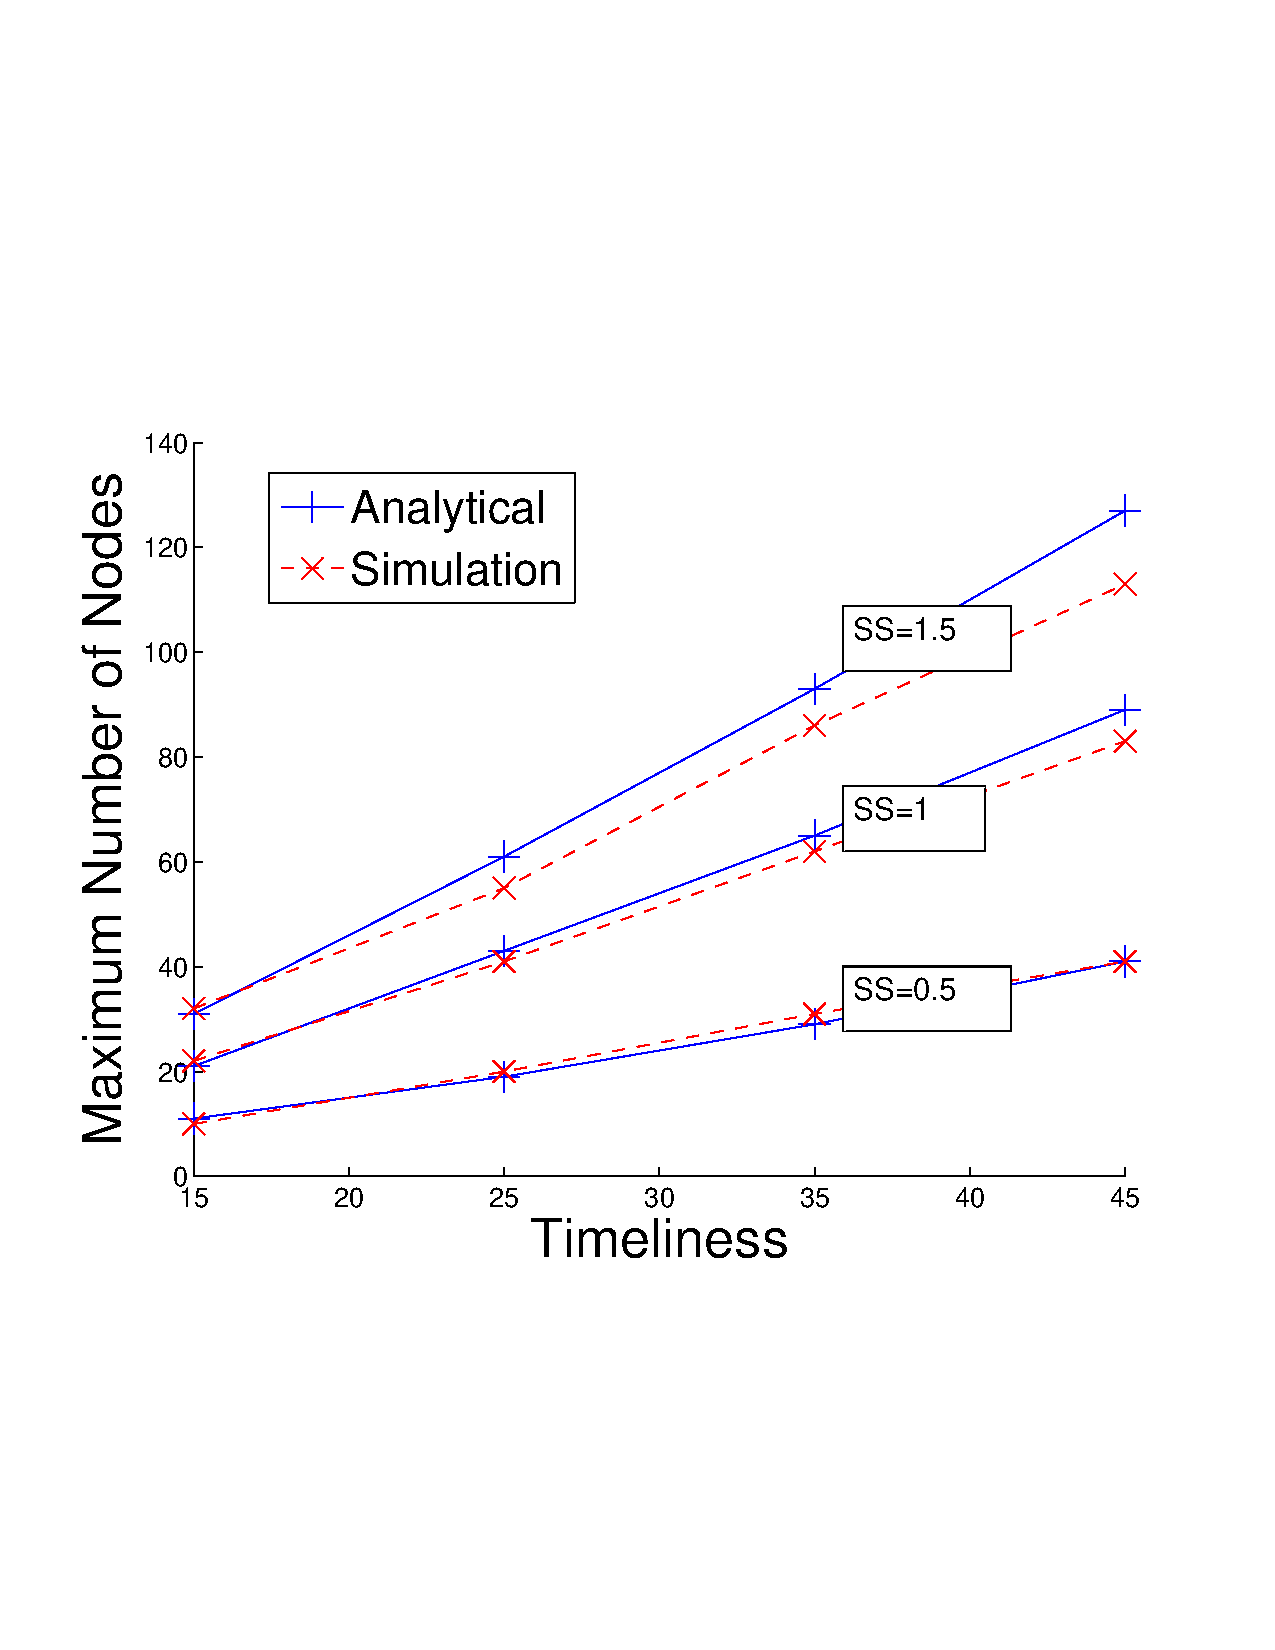
\includegraphics[scale=0.40, clip=true, trim=12mm 65mm 20mm 65mm]{figures/scal_sim_results/line_scal_anal_vs_sim_color.pdf}
%        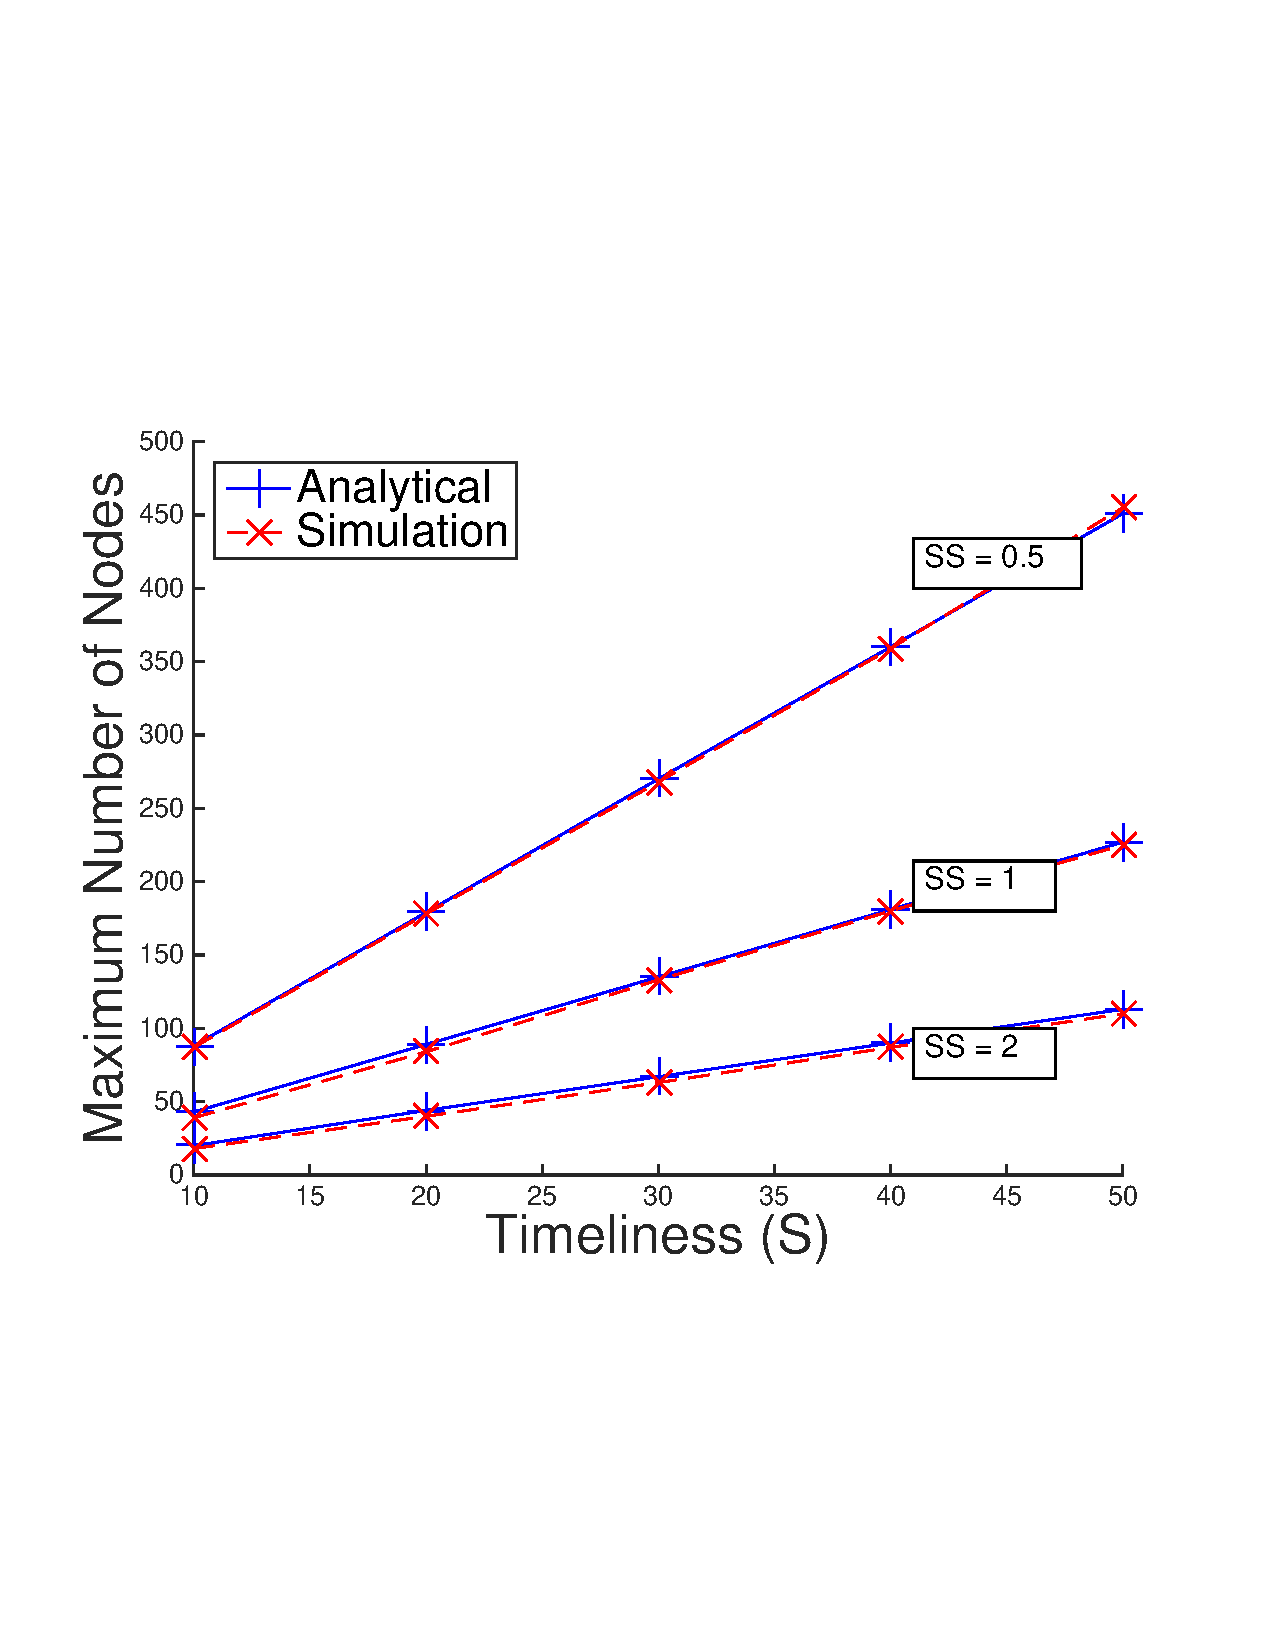
\includegraphics[scale=0.40, clip=true, trim=12mm 65mm 20mm 65mm]{figures/scal_sim_results/color_2d/line_uni_2d_qoi_vs_non_color_multiple.pdf}
        \label{fig:scal_vs_qoi_line}
        }
    \subfigure[Grid Network, $I_S = 48 KB$]{
%        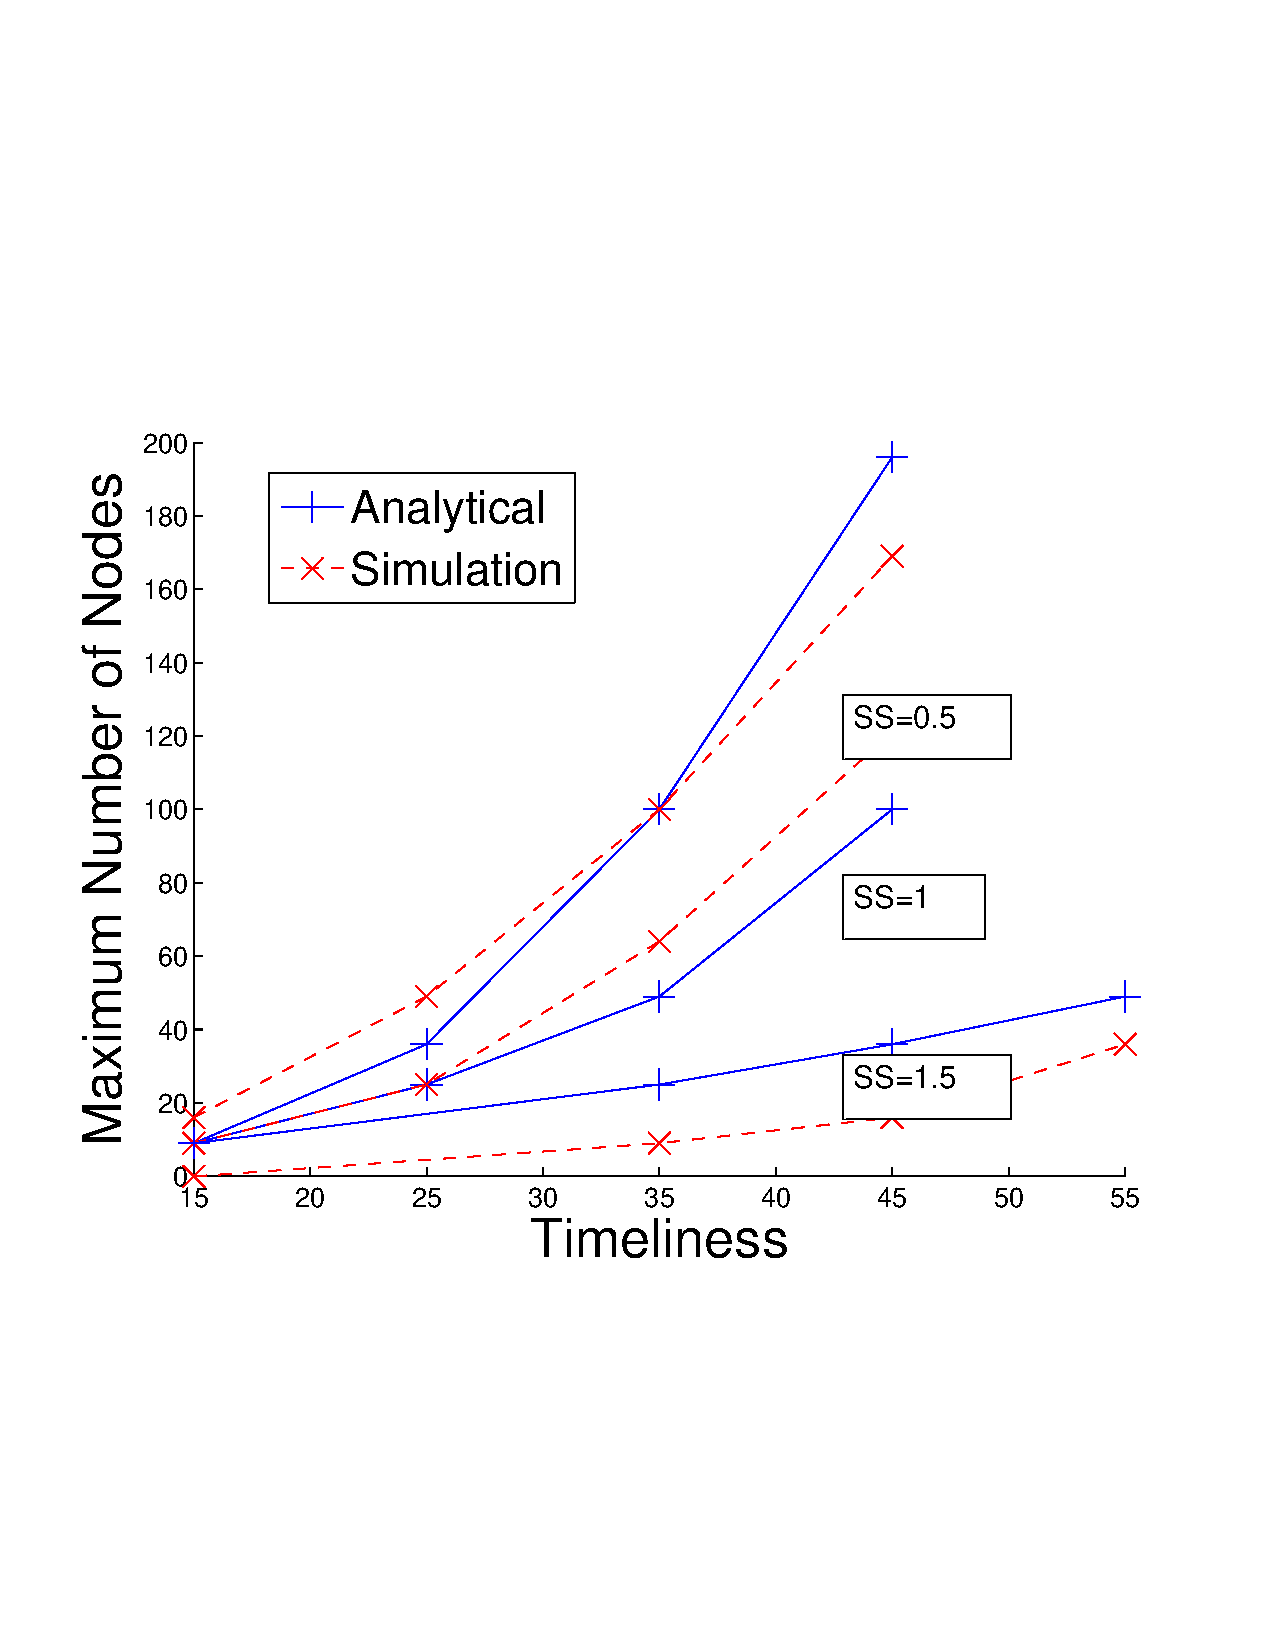
\includegraphics[scale=0.40, clip=true, trim=12mm 65mm 20mm 65mm]{figures/scal_sim_results/grid_scal_anal_vs_sim_color.pdf}
        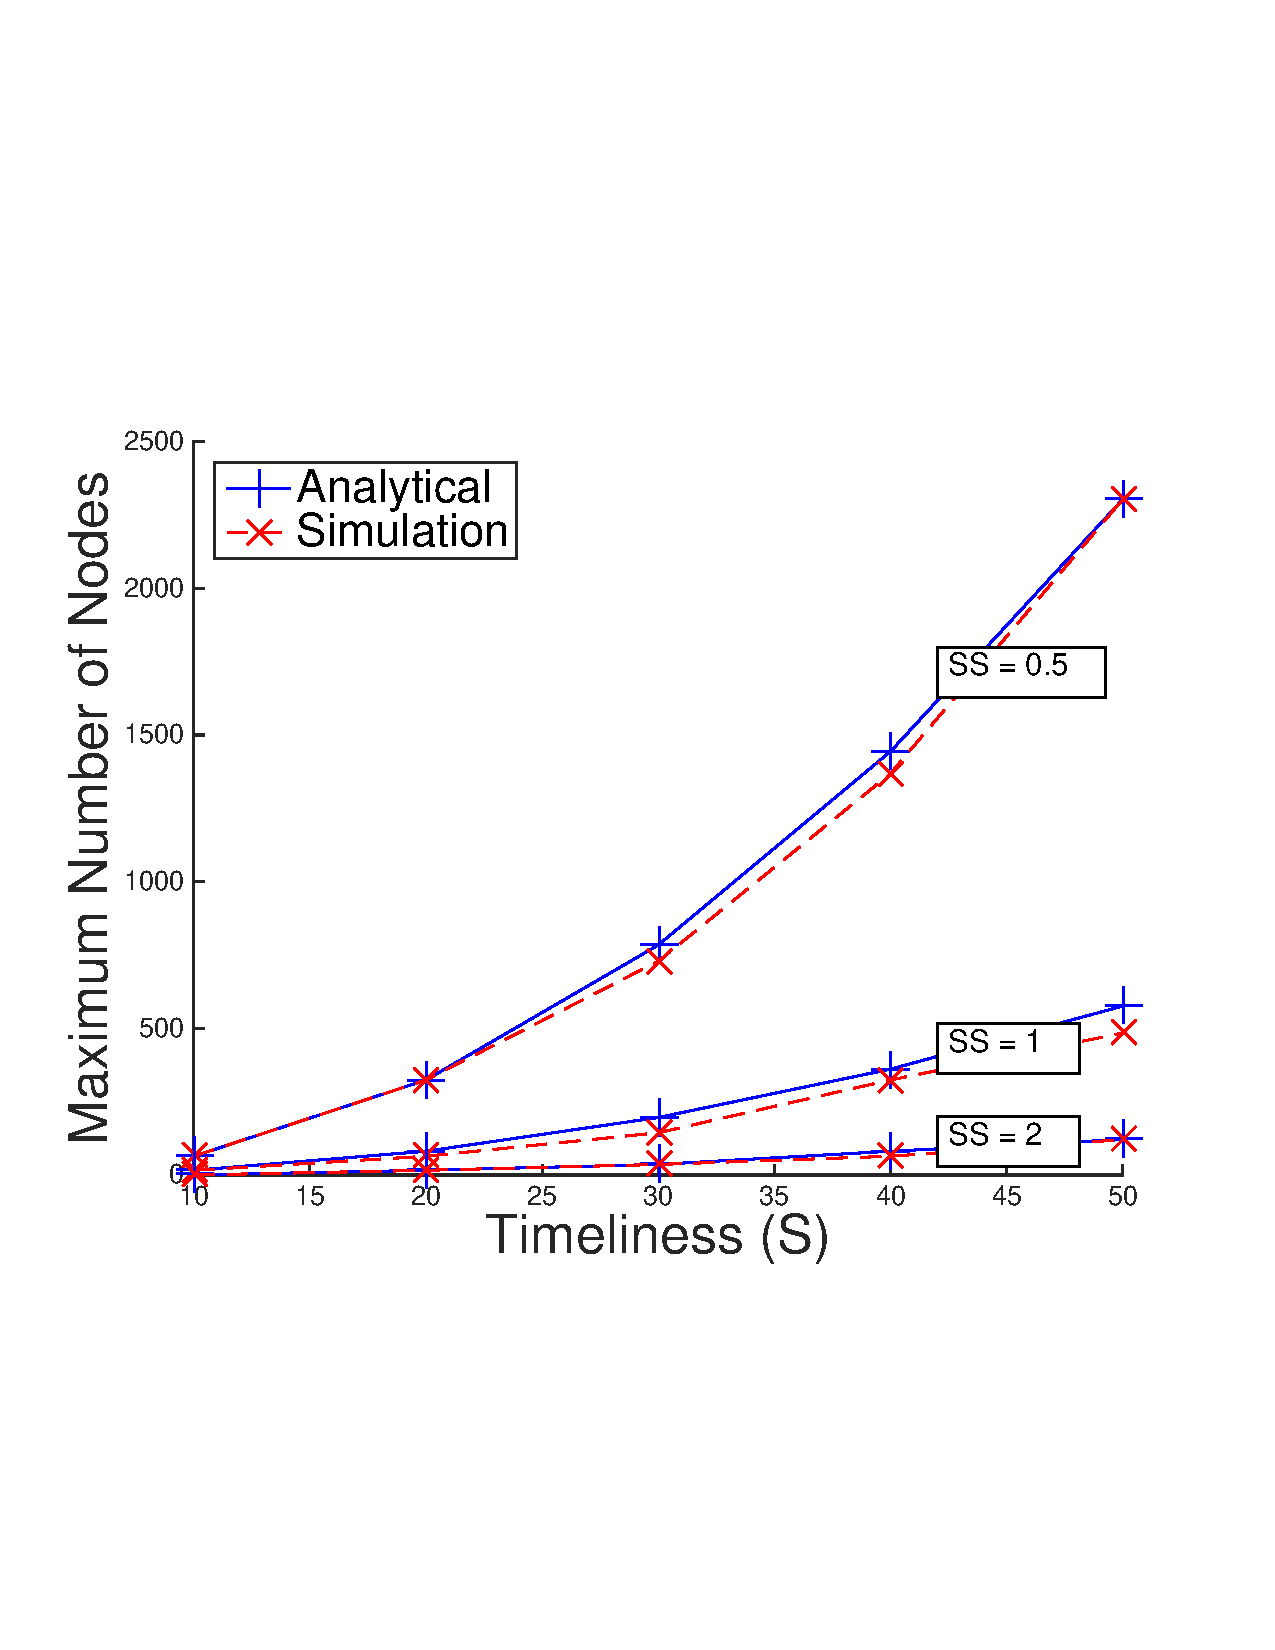
\includegraphics[scale=0.40, clip=true, trim=12mm 65mm 20mm 65mm]{figures/scal_sim_results/color_2d/grid_uni_2d_qoi_vs_non_color_multiple.pdf}
        \label{fig:scal_vs_qoi_grid}
        }
   \caption{Empirical results match analytical results closely for all tests.}
   \label{fig:scal_vs_qoi}
\end{figure}

To show how effective estimates using this framework can be, we simulated the network topologies and traffic described above in Section \ref{sec:example_applications} in the ns3 network simulator, comparing empirical results to those generated analytically with this framework, labeled \emph{Analytical}.  
%Due to space concerns, we only show a subset of results in Figure \ref{fig:scal_vs_qoi} to provide evidence of the effectiveness of the methodology.  All results generated, however, exhibit very similar trends of proximity between empirical and the analytical values.
We use a channel rate of $W= 2 Mbps$, packet sizes of $P_s = 1500$ bytes, and image sizes of $18$ and $48$ Kbytes.  As above, the correlation between Sum Similarity and $k_{req}$ is taken from the actual observed relation in Figure \ref{fig:topkSumSim}.  All values of parameters ($SS$, $T$, $I_S$, etc.) were chosen to test a variety of network sizes and QoI requirements while remaining within realistic network sizes, both with respect to real-world deployments and simulations with feasible run-times.

